\documentclass[10pt,twocolumn,letterpaper]{article}
\usepackage[review]{cvpr}
\usepackage{times,graphicx,amsmath,amssymb,booktabs,tabularx}
\usepackage[T1]{fontenc}
\usepackage{microtype}
\definecolor{cvprblue}{rgb}{0.15,0.43,0.64}
\usepackage[pagebackref,breaklinks,colorlinks,allcolors=cvprblue]{hyperref}
\def\paperID{Draft}
\def\confName{CVPR}
\def\confYear{2026}
\title{BrickAtlas: A Benchmark for Visual Evidence Following\\
with Paired LDraw Observations}
\author{Anonymous submission}
\begin{document}
\twocolumn[{
\renewcommand{\twocolumn}[1][]{#1}
\maketitle
\centering
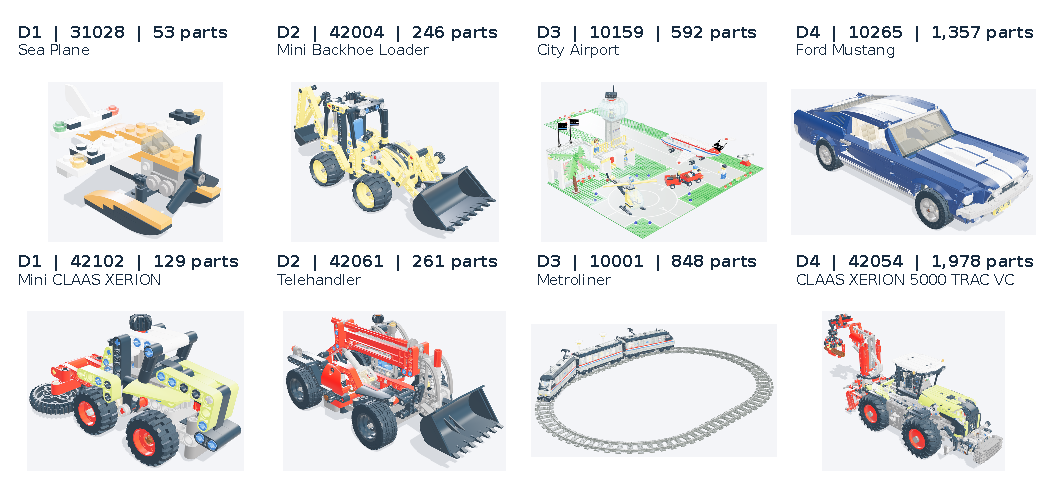
\includegraphics[width=\textwidth]{figures/source-overview.pdf}
\captionof{figure}{Real source assemblies across D1--D4 scale bands:
two examples per band, retaining original LDraw geometry and poses.
Source IDs and part counts connect each render to the released catalog.
These assemblies provide provenance. Figures~\ref{fig:complex-repair}--%
\ref{fig:complex-registration} develop source-backed repair, diagnosis
and registration problems. The supplement depicts all 24 sources
and the atomic visual controls.}
\label{fig:sources}
\vspace{12pt}
}]
\raggedbottom
\makeatletter
\setlength{\@dblfptop}{0pt}
\setlength{\@dblfpsep}{20pt}
\makeatother

\begin{abstract}
An answer can be correct without depending on the visual evidence that
the question selects. Evaluating this dependence requires observations
with controlled changes, unambiguous references, and a scoring protocol
that retains both successful and failed responses.
We present BrickAtlas, a benchmark built from 24 human-authored LDraw
assemblies containing 15,334 placed parts. Its primary visual track
contains 73 rendered-color pairs and 67 candidate-reference pairs;
67 position panels and 219 explicit text-graph observations provide
separate diagnostic controls. A display-local reference contract
distinguishes the object selected in the current image from its
historical source identity. Construction combines exact input records,
bounded answer-prior audits, and an independent human qualification
protocol. Evaluation reports endpoint accuracy, both-correct pair
accuracy, conditional adaptation, old-answer retention, and format
validity, with source and author dependence made explicit.
We provide a study design spanning proprietary and open-weight
vision--language models and text-only graph baselines.
Three separate compositional case studies demonstrate minimum repair,
adaptive fault diagnosis and rigid registration on real subassemblies.
The resource and deterministic audits are available; human
qualification and the proposed 15-model study remain pending.
Experiment tables specify the planned comparisons and leave all
unmeasured model results blank.
\end{abstract}

\section{Introduction}
Vision--language models often answer questions about small objects,
their appearance, and the references that identify them. Ordinary
accuracy measures whether an answer is correct on a supplied image.
It does not establish whether the model will remain correct when
the relevant evidence changes. A model may exploit answer frequency,
option position, a familiar source, or a stable reference convention.
A paired benchmark asks a more demanding question: can the model
answer both observations correctly under the same task contract?

Constructing such a benchmark introduces a second measurement problem.
The intervention must change the intended answer while preserving
what the question means. A part's source identifier can denote an
immutable record, whereas a label in an edited image can select a
different visible object. Without resolving this distinction, an
apparent failure to adapt may reflect an inconsistent question.
Similarly, a source record can certify a part type without proving
that the distinguishing geometry is visible to a human.

BrickAtlas addresses these problems through an auditable LDraw
resource~\cite{ldraw}. Source files provide exact geometry, transforms,
part types, and authorship. Rendered observations expose only the
evidence permitted by the question. Unique numeric labels, such as
B0035, identify image-local referents, while source identities remain
available to the evaluator. Every endpoint has a fixed question,
option list, image, gold answer, and provenance record.

The frozen primary benchmark has two atomic visual families.
\textbf{Color} is an appearance sanity check about the currently
rendered color of a single labeled part. Its paired intervention
changes appearance while keeping geometry and pose fixed.
\textbf{Part-type} asks which labeled candidate matches a target's
visible geometry. The target stays fixed while two candidate labels
exchange referents. This tests geometry matching together with
selection of the correct current label. We report the two families
separately because their visual requirements differ.
Beyond these controls, three newly designed examples combine graph
intervention, conditional inspection and spatial constraints on complete
source subassemblies. They illustrate richer task contracts and exact
ground truth, while remaining separate from the frozen visual study.

The evaluation connects three questions. First, is the answer
well defined in the exact observation? Second, can declared shallow
rules exploit construction regularities? Third, after these checks,
does paired performance reveal behavior hidden by ordinary accuracy?
The first two motivate construction and qualification; the third
motivates the planned experiments. A separate text-graph track
illustrates how matching low-level statistics can make a control more
informative, without treating graph performance as a visual score.

Our contributions are a source-backed paired resource with explicit
display semantics; a construction and qualification protocol linking
stimuli, references and review records; and an evaluation design
combining pair outcomes, legal input controls and clustered uncertainty.
Pair accuracy and controlled perturbations are established methods.
The intended value here is their auditable application to this
specific resource. Learned-model diagnostic value remains an empirical
question, rather than a conclusion of the construction process.

\section{Related Work}
\paragraph{Controlled visual reasoning.}
CLEVR~\cite{johnson2017clevr} and GQA~\cite{hudson2019gqa} connect
questions to explicit scene structure. VQA v2 uses similar images
with different answers to reduce language-only shortcuts~\cite{goyal2017vqa}.
Contrast sets probe local decision boundaries~\cite{gardner2020contrast},
and cycle-consistency studies answer stability under linguistic
variation~\cite{shah2019cycle}. BrickAtlas uses source structure to
construct and audit inputs while keeping source records outside
the primary visual request.

\paragraph{Paired evidence and reference grounding.}
Winoground evaluates joint image--text compatibility~\cite{thrush2022winoground}.
Its difficulty analysis highlights the need to distinguish intended
reasoning from visibility and other requirements~\cite{diwan2022winoground}.
Numeric-label selection is a restricted reference task compared with
natural referring expressions~\cite{mao2016refexp}.
VisualFLIP directly studies independently queried answer-changing
image pairs and competence-conditioned failures~\cite{zhu2026visualflip}.
Its v1 preprint reports 1,374 images, four perturbation categories and
24 MLLMs. BrickAtlas does not introduce paired correctness or claim
broader coverage. Its focus is the contract among source identity,
current display reference, restricted assignment audits and exact-input
human qualification.

\paragraph{Brick assembly and structural reasoning.}
BrickNet uses graph-backed assembly programs~\cite{kulits2026bricknet};
LEGO-Puzzles evaluates multistep spatial reasoning~\cite{tang2025legopuzzles};
PhyBlock studies physical understanding and planning~\cite{ma2025phyblock}.
BrickAtlas's current primary endpoint is atomic visual evidence
following. Its historical action dossiers and 3D replay support
inspection, but do not establish planning or physical execution
ability. The supporting graph construction instantiates a known
anonymous 1-WL limitation~\cite{xu2019gnn}, not a new expressivity theorem.

\section{Benchmark Definition}
\subsection{Resource, tracks and units}
The source resource contains 24 original assemblies, 15,334 placed
parts and 617 historical task dossiers. The paired visual benchmark
derives from 140 parents in that resource. A parent contributes one
A/B pair; a different image of the same parent is not a new source.
Table~\ref{tab:resource} separates primary observations, auxiliary
observations and historical material.

\begin{table}[t]
\centering\small
\caption{Resource units. Visual families are scored separately.
Graph change and invariance pairs share anchors. Historical
dossiers are not additional primary visual observations.}
\label{tab:resource}
\setlength{\tabcolsep}{3pt}
\begin{tabular}{@{}lrr@{}}
\toprule
Component & Parents & Observations\\
\midrule
Color & 73 & 146\\
Part-type & 67 & 134\\
Position panels (auxiliary) & 67 & 67\\
Hypothetical text graphs & 73 & 219\\
\midrule
Source assemblies & \multicolumn{2}{r}{24}\\
Placed source parts & \multicolumn{2}{r}{15,334}\\
Historical task dossiers & \multicolumn{2}{r}{617}\\
\bottomrule
\end{tabular}
\end{table}

Both visual families cover all 24 sources. Source bands D1--D4
describe assembly scale, not validated cognitive difficulty.
The supplemental source table reports each assembly and its
contribution. The historical dossier remains searchable and links
to 3D rotation, zoom, isolation, expansion and given-order replay.
These richer inspection views are not primary model inputs.

\subsection{Compositional case studies}
We include three source-backed examples, CX1--CX3, that require
multiple constraints to be satisfied jointly. They have public input
records, independently checkable GT and original-geometry renders.
These three examples are not an evaluated task family or evidence of
model difficulty. The supplement gives every question, adjacency,
coordinate and verification certificate.

\paragraph{CX1: multi-fault minimum repair.}
The 36-part backhoe subassembly of OMR 42004 induces 44 recognized
connector pairs and nine independent graph cycles.
Eight specified vertices become unavailable, splitting the supplied
graph into five components. The task asks for every minimum-cost
restoration that reconnects four terminal IDs, the final component
sizes, and whether a budget of two is sufficient.
It combines path reasoning, competing repairs and an optimality claim.
Exhaustive evaluation of all 256 subsets yields the unique minimum
$\{\mathrm{B0160},\mathrm{B0175},\mathrm{B0177}\}$, cost three,
and one 31-vertex final component. All 37 subsets with cost at most
two fail. Figure~\ref{fig:complex-repair} contracts only the surviving
components; the original graph remains the scored input.

\begin{figure*}[t]
\centering
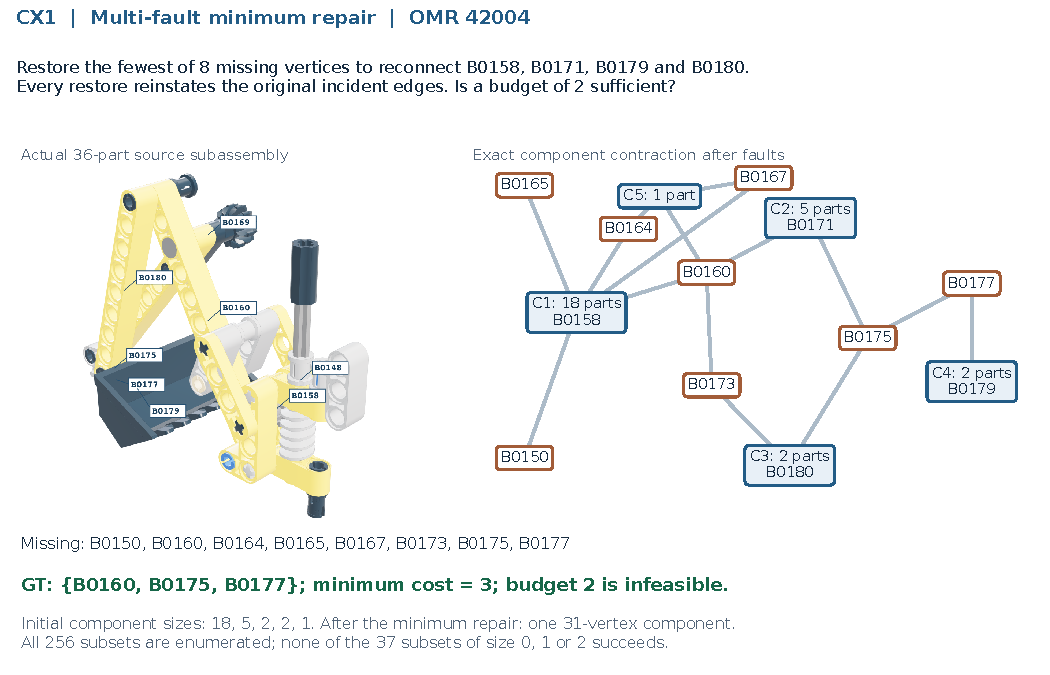
\includegraphics[width=\textwidth]{figures/complex-repair.pdf}
\caption{CX1: an original 36-part LDraw subassembly and a constrained
minimum-repair problem. Blue boxes summarize surviving components;
their terminal IDs and sizes are shown. Brown-bordered vertices are
unavailable candidates, with original incident edges retained in the
diagram for reasoning about restoration. GT requires a globally
minimal set, rather than any successful repair. The native 3D view
shows the intact source: faults are abstract graph interventions,
not simulated extraction or unsupported physical poses.}
\label{fig:complex-repair}
\end{figure*}

\paragraph{CX2: adaptive fault diagnosis.}
On the same source graph, four candidate worlds each disable three
vertices. Queries ask whether two IDs remain connected. The answer
must be a conditional policy that identifies the exact world with
minimum worst-case cost. Figure~\ref{fig:complex-diagnosis} gives
the hypotheses and computed policy: query Q3 first, then choose Q1
or Q2 from its outcome. The worst-case cost is two; no single binary
query can distinguish four worlds. Correctness is checked on every
world, not on one successful query sequence.

\begin{figure*}[t]
\centering
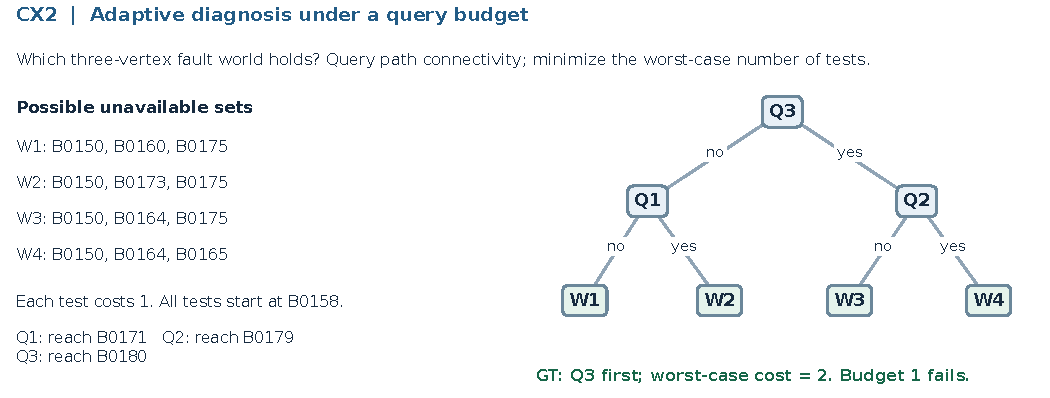
\includegraphics[width=\textwidth]{figures/complex-diagnosis.pdf}
\caption{CX2: minimum-cost conditional inspection. Each fault world
defines a different vertex-unavailability set on CX1's original graph.
Reachability outcomes are recomputed from that graph, not supplied as
an answer table. The optimal second query depends on the first result.
The tree is algorithmic GT; no model policy or physical sensor test
has been collected.}
\label{fig:complex-diagnosis}
\end{figure*}

\paragraph{CX3: correspondence and rigid pose recovery.}
Two actual 12-part axle assemblies in OMR 42061 instantiate the
same design at different source transforms.
Repeated part types admit four type-compatible anchor assignments.
The solver must determine the unique admissible correspondence,
fit a proper rigid transform, and transfer a probe's origin and
oriented local axis. Figure~\ref{fig:complex-registration} includes
all eight anchor coordinates and the probe.
Only one assignment admits maximum error below .05\,mm:
$R=\operatorname{diag}(-1,1,-1)$ and $t=(16,0,120)$\,mm.
All twelve complete source part transforms verify this result.
The other assignments violate pairwise-distance bounds, so their
rejection does not depend on a particular numerical optimizer.

\begin{figure*}[t]
\centering
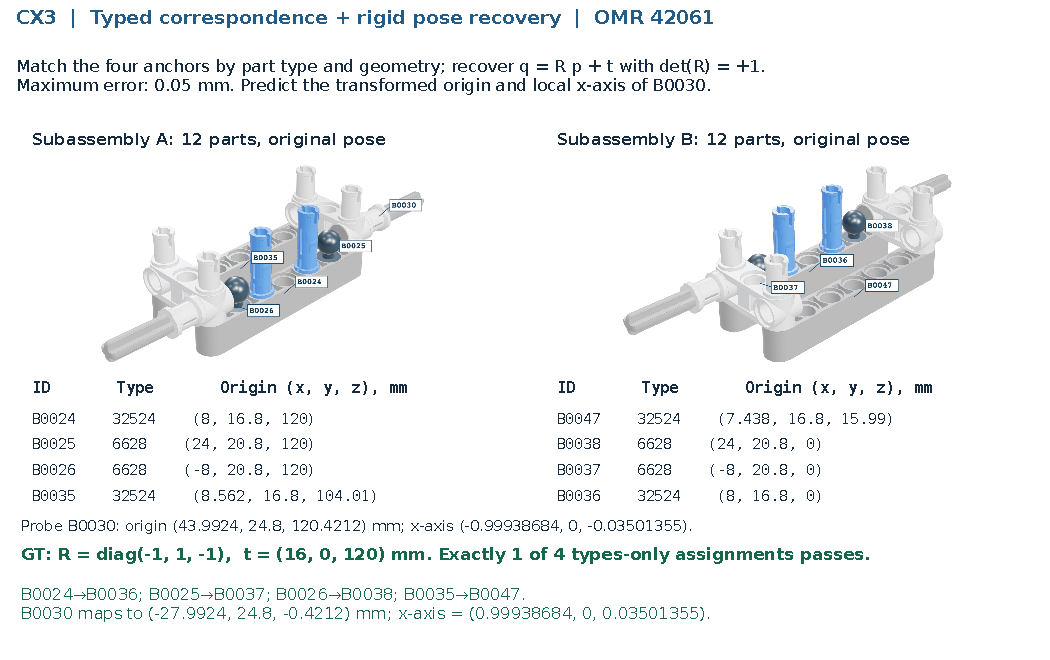
\includegraphics[width=\textwidth]{figures/complex-registration.pdf}
\caption{CX3: two complete source axle assemblies, duplicated part
types, four-anchor matching, proper rigid registration and probe
transfer. Source geometry and all internal poses are preserved.
Coordinates specify part origins in world millimeters.
GT includes correspondences, rotation, translation, transformed
probe location and direction. These source-data constraints go
beyond choosing one matching part or identifying an appearance.}
\label{fig:complex-registration}
\end{figure*}

The examples have no learned-model or human results and are not
added to the 140 paired visual tests. Their complexity is specified
by operations and constraints, not inferred from source-scale bands.
Graph connectivity is an explicit abstraction; the examples make
no claim about physical removal paths, clutch forces or stability.

\subsection{Source identity and current display reference}
Let $c=(h,i)$ identify a source instance by source-file hash $h$
and part ID $i$. Its record $T(c)$ contains the original type,
color and transform. For observation $o$, the display mapping
$d_o(\ell)$ selects the object marked by label $\ell$.
The answer $y_o$ follows the current question and $d_o$, rather
than necessarily retrieving a property from $T(c)$.

Every visual question explicitly states that references select
objects in the supplied image, that appearance or label assignments
may be edited, and that the answer must follow the current image.
The model returns one JSON object with a listed \texttt{choiceId}.
Canonical records, intervention metadata, golds and pair membership
remain evaluator-only.

For Color, the question is ``What color is the object currently
marked B0035 in this image?'' For Part-type, it asks which displayed
candidate label currently marks an object with the same visible part
geometry as the target, ignoring color and pose. A label reassignment
changes the latter answer without changing a canonical part's type.
The schema key \texttt{shape-match} refers to this Part-type family.

\subsection{What each observation permits}
A primary input contains the complete system/user text, four options
and one native 1280$\times$800 PNG. A and B are independent requests;
neither includes the counterpart, its answer or conversational history.
External crops, source records, masks and tools are excluded from
the primary visual condition. Provider image policy and generation
settings belong to the study configuration.

The source geometry and saved poses remain unchanged. Operand-only
views can omit surrounding support and therefore represent observations
of parts, not freestanding assemblies. Expansion similarly supports
inspection. Recognized connector graphs and preserved source meshes
do not certify complete mating, collision-free insertion or stability.
The resource retains 573 intersection candidates requiring physical
review; the present visual benchmark does not resolve those judgments.

\section{Construction and Qualification}
\subsection{Controlled visual changes}
\paragraph{Color.}
Each of 73 pairs renders one operand and one label. Only the body-color
parameter changes between two distinct named opaque colors; geometry,
source pose, camera, scale, visibility and label projection stay fixed.
Across 146 endpoints the displayed golds are Red, Blue, Yellow and
Black with counts 37, 37, 36 and 36. All pairs have zero changed pixels
outside the common projected body mask with one pixel of antialiasing
dilation. Three independently regenerated canaries are byte-identical.
These are construction checks, not human color judgments.

Color is an appearance sanity track. A legal whole-image color
baseline receives only the current PNG and text/options, without a
mask, source record or counterpart. Its frozen thresholds yield
141/146 correct endpoints, five abstentions, and 68/73 Both.
This confirms that the track can be solved largely by rendered
appearance; it does not test reference selection among multiple parts.

\paragraph{Part-type.}
Each of 67 pairs retains the target and underlying geometry while
swapping the labels of the matching candidate and a nonmatching
candidate. The option list is fixed within the pair. Geometry pixels
match exactly, and pixel changes lie within the label masks.
Two independently regenerated canaries are byte-identical.
Source part-type equality derives a candidate gold; whether exactly
one match is visually identifiable is checked separately by humans.

The 67 auxiliary position panels display a target and four candidate
panels without text embedded in the image. Options refer to candidate
positions. The comparison changes reference interface, separation
and visual access together, so it cannot isolate a causal OCR effect.
Panels have their own human decisions and do not enter paired Both.

\subsection{Assignment and restricted shortcut audits}
Candidate construction enumerates four-option permutations and
admissible nonmatching swaps with visible anchors and a unique source-type
match. For Part-type, 4,824 candidates reduce to 2,412 constraint-equivalent
configurations. A finite assignment selects one per parent under
precommitted bounds: each arm has 16 or 17 golds per option position;
each off-diagonal A-to-B transition has five or six pairs; diagonal
transitions have zero pairs.

Every fixed-choice rule is bounded by .30 equal-source endpoint
accuracy. Thirteen declared oracle-A rules are bounded by .40 B
accuracy in both micro and equal-source estimates. These privileged
audits receive the correct A answer; some also receive A-side source
geometry. They inspect option order, label numbers or spatial
relations, without reading B pixels. They are construction diagnostics,
not legal single-image baselines or upper bounds on models.

The frozen first-alternative rule attains 23/67 Both. Because each
transition cell has at most six pairs, any fixed mapping from A choice
alone to B choice has in-sample B accuracy at most $24/67$.
Additional features fall outside that bound. Color was not jointly
optimized, and its strongest declared oracle rules reach 32/73.
The full transition matrices and rule outputs remain public.

\subsection{Exact-input independent human qualification}
All 347 visual observations are frozen before qualification. Each
receives two judgments from six distinct reviewers. A reviewer sees
at most one observation of a parent, including the auxiliary panel;
A/B reviewer sets are disjoint. Queues show one exact observation
with native pixels, while hiding the source record, gold, condition,
pair membership, other reviews and model outputs.

Reviewers provide a visual choice, one of decidable/ambiguous/
unanswerable/contradictory, and checks for unique target reference,
unique visible answer, sufficient visibility and absence of reference
contradictions. They attest to native-size inspection and independence.
Any decision, choice or structured-check disagreement requires
an additional independent adjudicator. A final decidable choice
in conflict with generated gold returns the observation for revision
and renewed qualification; gold is not silently replaced.

The protocol requires a final decision for every planned visual
endpoint before collection. All endpoints remain in the full
denominator; an additional qualified subset contains pairs with
two finally decidable endpoints. Raw agreement, choice/check agreement,
kappa, exclusions and source coverage are reported. At present, no
genuine human judgments have been collected, so answerability is an
open acceptance requirement. Machine consistency does not satisfy it.

\section{Evaluation Metrics}
\subsection{Correctness, adaptation and validity}
For $N$ fixed pairs, let $p_{Ai},p_{Bi}$ be normalized predictions,
$y_{Ai}\ne y_{Bi}$ the gold choices, and $v_{Ai},v_{Bi}$ valid-format
indicators. Invalid or missing output never matches a gold. Define
\begin{align}
\mathrm{AAcc}&=\frac{1}{N}\sum_i[p_{Ai}=y_{Ai}],\\
\mathrm{NewAcc}&=\frac{1}{N}\sum_i[p_{Bi}=y_{Bi}],\\
\mathrm{Both}&=\frac{1}{N}\sum_i[p_{Ai}=y_{Ai}][p_{Bi}=y_{Bi}].
\end{align}
Both is the primary pair outcome. AAcc exposes baseline competence;
NewAcc exposes performance on the changed observation. Micro
conditional adaptation divides the both-correct count by the A-correct
count. A zero denominator is undefined, not zero.

Old-gold retention is $N^{-1}\sum_i v_{Bi}[p_{Bi}=y_{Ai}]$.
Together, new-gold correctness, old-gold retention, other valid wrong
answers and invalid B output partition the B outcomes. Retention is
an observed answer pattern, not evidence of an internal memory mechanism.
We report valid A, valid B and valid-both rates alongside semantic
metrics. Stable invalid strings do not count as semantic consistency.

The supplemental Part-type example has GT token pair $(C,D)$.
Only matching both tokens earns
Both=1. Returning the A gold on B instead contributes to old-gold
retention. These statements define the scorer; no displayed GT is
a claimed model response.

\subsection{Aggregation and uncertainty}
For outcome $z_{si}$ from pair $i$ of source $s$, the primary estimator is
\begin{equation}
\widehat{\mu}_{\mathrm{source}}=
\frac{1}{|S|}\sum_{s\in S}\frac{1}{n_s}\sum_{i=1}^{n_s}z_{si}.
\end{equation}
Micro rates and eligible pair/source counts accompany it. Conditional
source rates are computed within sources with A-correct pairs, then
averaged; they are not the ratio of two source-macro scores.
Descriptive 95\% intervals use 10,000 whole-source bootstrap draws
with seed 20260920. Paired model differences use the same items.

Sources share authors and common parts. Sensitivity analysis uses
18 primary-author groups and 17 contributor-connected groups, reporting
equal-author means, clustered intervals and leave-one-author-out
differences. Full and qualified-subset results are reported together;
their difference uses shared source resampling and recomputes each
mean on its eligible sources. Empty subsets remain undefined.
Exact rational point comparisons retain ties in AAcc and Both ranks.
Rank reversals and unadjusted pairwise intervals are exploratory.
Intervals crossing zero do not support a directional ranking.

\subsection{Requests, failures and repeat policy}
Every scheduled request retains its input hash, pre-call intent,
provider receipt or explicit failure, normalized answer and inclusion
record. Refusals, timeouts, API failures, malformed outputs and missing
receipts remain incorrect in the planned denominator. Absent calls
cannot disappear through filtering. Repeated invocations, if collected,
must all be retained under a frozen policy; source intervals alone
do not measure cross-call variation. The existing evaluator implements
a sealed three-model, one-attempt study. The broader proposal below
requires a new version with its own adapters and complete run manifest.

\section{Planned Experiments}
\subsection{Research questions and model coverage}
We organize the study around three questions:
(i) does Both reveal differences not apparent in AAcc;
(ii) how do image withdrawal, qualification and reference interface
affect those differences; and (iii) do structural controls distinguish
behavior that natural graph accuracy obscures?
No model outcome is assumed by these questions.

Table~\ref{tab:models} proposes 15 distinct models: seven proprietary
VLMs, six open-weight VLMs and two open-weight text-only models.
The inventory follows the repository's September 20, 2026 planning
snapshot; it is not a claim of current endpoint availability.
Model revision, provider, precision, image processing and collection
window must be checked and committed before execution. A hosted
open-weight endpoint is a specific service configuration, not
automatically equivalent to its original weights.

\begin{table*}[t]
\centering\small
\caption{Proposed model inventory. Names and classes are planning
metadata; no row represents a completed run. VLMs receive visual,
no-image and graph conditions; text-only models receive explicit graphs.
The two effort contrasts in Table~\ref{tab:modes} are configurations,
not additional models.}
\label{tab:models}
\begin{tabular}{@{}lll@{}}
\toprule
Model & Model class & Planned inputs\\
\midrule
GPT-6 Astra & Proprietary VLM & Visual / no-image / graph\\
GPT-5.6 Sol & Proprietary VLM & Visual / no-image / graph\\
GPT-5.6 Luna & Proprietary VLM & Visual / no-image / graph\\
Claude Fable 5.1 & Proprietary VLM & Visual / no-image / graph\\
Claude Sonnet 5 & Proprietary VLM & Visual / no-image / graph\\
Gemini 3.1 Pro Preview & Proprietary VLM & Visual / no-image / graph\\
Gemini 3.8 Flash & Proprietary VLM & Visual / no-image / graph\\
Qwen3.5-9B & Open-weight VLM & Visual / no-image / graph\\
Qwen3.5-27B & Open-weight VLM & Visual / no-image / graph\\
InternVL3.5-8B & Open-weight VLM & Visual / no-image / graph\\
InternVL3.5-38B & Open-weight VLM & Visual / no-image / graph\\
Gemma 3 4B IT & Open-weight VLM & Visual / no-image / graph\\
Gemma 3 27B IT & Open-weight VLM & Visual / no-image / graph\\
Qwen3-32B & Open-weight text LM & Graph\\
DeepSeek-R1-Distill-Qwen-32B & Open-weight text LM & Graph\\
\bottomrule
\end{tabular}

\end{table*}

Access is planned through a mixture of hosted APIs and self-hosting.
The budget snapshot lists 12 models on OpenRouter and three for
self-hosting; listing alone does not verify live account access,
image delivery or backend revision stability. We compare advertised
model classes without assigning a universal ``reasoning/nonreasoning''
label to proprietary systems. Only supported, explicitly frozen
thinking or effort modes enter the mode comparison.

\subsection{Primary visual results and error decomposition}
Table~\ref{tab:visual} reserves the primary result matrix.
Each cell will report an equal-source percentage, with micro rates,
counts and clustered intervals in accompanying records. All models
receive the same frozen observations and options. Color and Part-type
remain separate, including in model comparisons.

\begin{table*}[t]
\centering\small
\caption{Planned primary visual results (\%, equal-source).
A and New are endpoint accuracy; Both requires both endpoints correct.
All result cells are intentionally empty. Companion records will
include micro scores, denominators and source intervals.}
\label{tab:visual}
\setlength{\tabcolsep}{8pt}
\begin{tabular}{@{}lrrrrrr@{}}
\toprule
Model & \shortstack{Color\\A} & \shortstack{Color\\New} & \shortstack{Color\\Both} & \shortstack{Part-type\\A} & \shortstack{Part-type\\New} & \shortstack{Part-type\\Both}\\
\midrule
GPT-6 Astra &  &  &  &  &  & \\
GPT-5.6 Sol &  &  &  &  &  & \\
GPT-5.6 Luna &  &  &  &  &  & \\
Claude Fable 5.1 &  &  &  &  &  & \\
Claude Sonnet 5 &  &  &  &  &  & \\
Gemini 3.1 Pro Preview &  &  &  &  &  & \\
Gemini 3.8 Flash &  &  &  &  &  & \\
Qwen3.5-9B &  &  &  &  &  & \\
Qwen3.5-27B &  &  &  &  &  & \\
InternVL3.5-8B &  &  &  &  &  & \\
InternVL3.5-38B &  &  &  &  &  & \\
Gemma 3 4B IT &  &  &  &  &  & \\
Gemma 3 27B IT &  &  &  &  &  & \\
\bottomrule
\end{tabular}

\end{table*}

Table~\ref{tab:diagnostics} separates successful adaptation from old-gold
retention and invalid output. Conditional adaptation must be read
with AAcc and eligible counts. Otherwise a model correct on very few
A endpoints could appear strong after conditioning.
The full B partition, including other-wrong and invalid, will accompany
the compact table. Differences attributable primarily to format or API
failures limit a semantic interpretation.

\begin{table*}[t]
\centering\small
\caption{Planned response diagnostics (\%, equal-source).
Adapt.: B correctness conditional on A correctness, with eligible
counts reported separately. Old: old-gold retention. Valid:
both endpoints have valid format. Cells remain empty pending inference.}
\label{tab:diagnostics}
\setlength{\tabcolsep}{7pt}
\input{generated/diagnostics.tex}
\end{table*}

\subsection{Image dependence, qualification and interface controls}
The no-image condition removes only the image content from each
visual request. The 140 stripped A/B pairs have identical messages
and different golds. An identical deterministic prediction therefore
has Both=0 and symmetric endpoint accuracy at most one half.
Independent stochastic calls can produce different answers, so this
identity does not force every real no-image run to score zero.
The condition tests image dependence, not specific reference selection.

Table~\ref{tab:controls} records no-image Both, separate panel accuracy
and qualified-minus-full changes. Image-minus-no-image paired differences
are derived alongside it. A change after qualification must be read
with exclusions and source coverage. The panel comparison is descriptive
because layout and visual access also change.
The current Part-type track has no separately qualified visual
answer-preserving intervention. It supports candidate-reference
reassignment claims; broader robustness to irrelevant visual changes
would require a new control and renewed qualification.

\begin{table*}[t]
\centering\small
\caption{Planned controls. No-image and panel entries are percentages;
QA--full entries are percentage-point differences in Both between
the both-decidable subset and full set. ``Type'' denotes Part-type.
All measured entries remain empty.}
\label{tab:controls}
\setlength{\tabcolsep}{6pt}
\begin{tabular}{@{}lrrrrr@{}}
\toprule
Model & \shortstack{No-image\\Color Both} & \shortstack{No-image\\Type Both} & \shortstack{Panel\\accuracy} & \shortstack{Color\\QA--full} & \shortstack{Type\\QA--full}\\
\midrule
GPT-6 Astra &  &  &  &  & \\
GPT-5.6 Sol &  &  &  &  & \\
GPT-5.6 Luna &  &  &  &  & \\
Claude Fable 5.1 &  &  &  &  & \\
Claude Sonnet 5 &  &  &  &  & \\
Gemini 3.1 Pro Preview &  &  &  &  & \\
Gemini 3.8 Flash &  &  &  &  & \\
Qwen3.5-9B &  &  &  &  & \\
Qwen3.5-27B &  &  &  &  & \\
InternVL3.5-8B &  &  &  &  & \\
InternVL3.5-38B &  &  &  &  & \\
Gemma 3 4B IT &  &  &  &  & \\
Gemma 3 27B IT &  &  &  &  & \\
\bottomrule
\end{tabular}

\end{table*}

\subsection{Text-graph reasoning and algorithmic controls}
The supporting task asks for the number of connected components
after deleting a named node from an explicit undirected graph,
counting isolated survivors. The natural inventory has 73 questions.
The hypothetical set contains 73 anchors, 73 answer-changing
partners and 73 isomorphic answer-preserving partners.

Twelve strong change pairs across eight sources match surviving
nodes, edge count, target degree, complete degree multiset and isolate
count. They compare a six-cycle with two triangles, plus identical
isolates. The other 61 pairs across 23 sources are degree-visible
controls. Their invariance partners are reported separately.
These hypothetical edge lists are not newly inferred physical connections.
The supplement shows a complete strong example and its independently
recomputed component-count GT. CX1--CX2 instead use a larger induced
source graph and require optimization or a conditional policy; those
examples remain outside the planned graph result matrix.

Deterministic audits already establish the relevance of this partition.
An isolates-plus-one heuristic solves 72/73 natural questions and
61/61 degree-visible change pairs, but 0/12 strong change pairs.
BFS and union-find solve all. Anonymous uniform-feature 1-WL cannot
distinguish the two strong endpoints; a predictor restricted to that
signature must return the same answer to different golds.
This restriction excludes unique-ID, positional and higher-order
features and does not describe a trained language model's internals.
The supplement reports the full algorithm audit.

Table~\ref{tab:graph} reserves learned-model results for all four
partitions. Both and symmetric endpoint accuracy are computed
within each partition; the compact table shows Both. A repeated
wrong answer on invariance is not success. Shared anchors prohibit
counting these partitions as independent datasets. The strong subset
is a small construction challenge, not a broad graph-reasoning benchmark.

\begin{table*}[t]
\centering\small
\caption{Planned text-graph results. The four partition columns
report equal-source Both (\%); symmetric endpoint accuracy and
partition-specific valid-both rates accompany the full records.
Format valid reports valid predictions over 219 distinct observations.
No model results have been entered.}
\label{tab:graph}
\setlength{\tabcolsep}{5pt}
\input{generated/graph.tex}
\end{table*}

\subsection{Reasoning modes and staged collection}
Table~\ref{tab:modes} reserves two within-model contrasts: Qwen3.5-27B
thinking off/on and Gemini Pro lower/higher effort. The comparison
must retain exact supported settings and include billed hidden
reasoning in token and cost accounting. Its differences are computed
on identical items with all scheduled outputs retained. The stated
modes remain proposals until the adapters verify their support.

\begin{table*}[t]
\centering\small
\caption{Planned mode contrasts. Score differences are percentage
points; output tokens and USD summarize each configuration in the
contrast. Both configurations must be reported, with their exact
settings. Empty cells indicate unmeasured quantities.}
\label{tab:modes}
\setlength{\tabcolsep}{5pt}
\begin{tabular}{@{}lrrrrr@{}}
\toprule
Configuration contrast & $\Delta$ Color & $\Delta$ Type & $\Delta$ Strong & \shortstack{Output\\tokens} & USD\\
\midrule
Qwen3.5-27B: thinking on minus off &  &  &  &  & \\
Gemini 3.1 Pro: higher minus lower effort &  &  &  &  & \\
\bottomrule
\end{tabular}

\end{table*}

An initial MVP keeps all 15 models while reducing observations:
12 complete pairs per visual family, their 12 Part-type panels,
the corresponding 60 no-image requests, and 54 graph observations.
It retains all 12 strong graph parents and six degree-visible parents.
One invocation per configuration yields 2,370 requests; the two
additional mode configurations raise this to 2,718.
Selected IDs, source coverage, subset priors and exact-input
qualification must be frozen before any live run. The new provider
adapters and subset qualification gate are not yet implemented.
This MVP validates delivery, cost and exploratory failure patterns;
it does not provide a stable full-dataset ranking.

\section{Limitations and Release}
BrickAtlas covers two atomic visual families and a small public
source collection. Color does not address natural color constancy,
and candidate-label reassignment does not establish general referring
expression comprehension. CAD equality does not guarantee visible
uniqueness. Physical buildability, continuous insertion and dynamics
are outside the present evaluation. Public source reuse also leaves
contamination and dependence concerns.

The release includes source attribution, exact observation manifests,
frozen assignment records, reviewer packages, deterministic audits,
scoring code and a 3D inspection interface. Current paper assets
and blank experiment tables are generated from an explicit proposal
schema; earlier manuscripts and revision material are archived.
The existing three-model protocol and the new 15-model proposal
are distinct studies. No old response is transferred to a new stimulus.

Human qualification and learned-model evaluation remain unfinished.
Useful diagnostic value would require paired differences that survive
the declared input controls, qualification analysis and dependence
checks. If Both merely reproduces ordinary-accuracy rankings, or
effects are explained by failures and visibility, the interpretation
must reflect that outcome. The current release establishes an
auditable resource and a concrete experiment design, with the
empirical comparisons left open.

\clearpage
{\small
\bibliographystyle{ieeenat_fullname}
\bibliography{references}
}
\end{document}
